\documentclass{beamer}
% adaptation au français et accents
\usepackage[utf8]{inputenc}
\usepackage[T1]{fontenc}

% insérer des images et graphiques
\usepackage{graphicx}
%Thème
%\usetheme{Warsaw}
% couleurs
\usepackage{xcolor}
%theme de ses morts


%##########################################################

\begin{document}

\title{Projet Scientifique Informatique}
	\subtitle{L2 Informatique \\
	Modèle d'évacuation en cas urgence  }
	\author {Romain Kugler \& Yann Martin D'Escrienne}
	\institute{Université Nice-Sophia Antipolis}
	\date{2019}
	
%Affiche le titre ci-dessus	
\begin{frame} \titlepage \end{frame}

%Intro
\begin{frame}
	\frametitle{Introduction}
	\framesubtitle{Contexte}
	
	\begin{block}{}
	\begin{itemize}
		\item \textbf{De quoi s'agit-il ?} \\
		Modélisation d'évacuation en cas d'urgence\\
		\item \textbf{Qui ?}\\
		Individus de tout âges et milieux sociaux \\
		\item \textbf{Où ?}\\
		Salle de cinéma, amphithéâtre, bureaux...\\
		\item \textbf{Quels dangers ?}\\
		Feu, Fumée, Attentats...
	\end{itemize}
	\end{block}	
\end{frame}



%Problématique
\begin{frame}
	\frametitle{Problématique}
	\framesubtitle{Identifier les problèmes}
	
	\begin{block}{\textbf{Quels enjeux?}}
	\begin{itemize}
		\smallskip
		\item Limiter les pertes humaines	
	\end{itemize}
	\end{block}
	
	\medskip
	
	\begin{block}{\textbf{Comment optimiser une évacuation?}}
	\begin{itemize}
		\medskip
		\item Identifier les \textbf{paramètres importants}
		\smallskip 
		\item \textbf{Temps} d'évacuation \textbf{minimal}\\
	\end{itemize}
	\end{block}
	
	\medskip
	
	\begin{block}{\textbf{\textcolor{red}{Quelle est la relation entre le temps d'évacuation et ces différents paramètres?}}}
	\end{block}	
	
\end{frame}


%Modélisation


\begin{frame}
	\frametitle{Modélisation}
	\framesubtitle{Choix des paramètres et des mesures}
	\begin{block}{\textbf{Paramètres}}
	\begin{itemize}
		\medskip
		\item \textbf{Densité} d'individus dans la salle\\
		\item Nombre de \textbf{sorties}\\
		\item \textbf{Vitesse} de déplacement\\
		\item \textbf{Obstacles}\\
	\end{itemize}
	\end{block}
	
	\bigskip
	
	\begin{block}{\textbf{Mesures}}
	\begin{itemize}
		\medskip
		\item \textbf{Temps} d'évacuation totale \\
		\item \textbf{Pourcentage d'individus} évacués au temps T\\
	\end{itemize}
	\end{block}
\end{frame}

\begin{frame}
	\frametitle{Modélisation}
	\begin{block}{\textbf{Hypothèse simplificatrice}}
	\medskip
	\begin{itemize}
		\item Monde en 2D, case par case 
		\item Feu, individus, obstacles,.. occupent une case
		\item Les individus ont la même vitesse de déplacement 
	\end{itemize}
	\end{block}
\end{frame}

\begin{frame}
	\frametitle{Modélisation}
	\framesubtitle{Premier jet sur Netlogo}
	
	
	\begin{figure}
	\bigskip
  		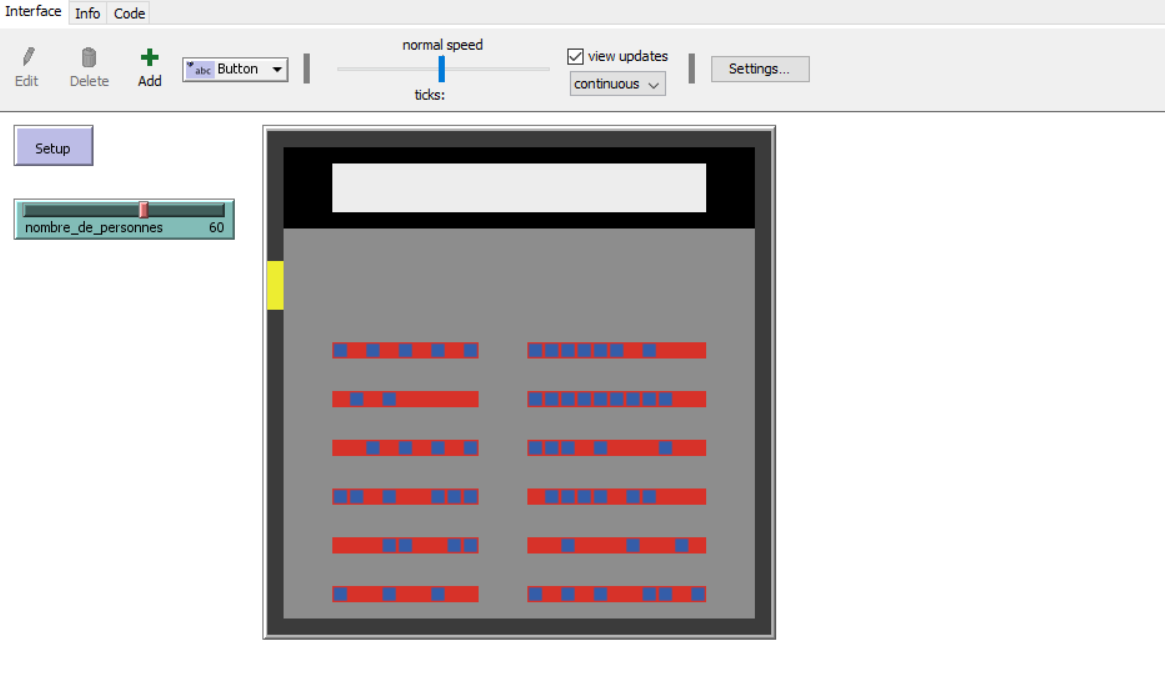
\includegraphics[width=\linewidth]{Cine_Setup.PNG}
 		\caption{Salle de cinéma générée sur Netlogo}
 		\label{pic: cine}
\end{figure}
	
\end{frame}




%Résultats attendus
\begin{frame}
	\frametitle{Résultats attendus}
	
	\begin{block}{\textbf{Mettre en valeur l'importance de certains paramètres}}
	\begin{itemize}
	\item Nombre et localisation des sorties
	\item Disposition des obstacles
	\end{itemize}
	\end{block}
	
	\bigskip
	
	\begin{block}{\textbf{Faire varier des paramètres}}
	\begin{itemize}
	\item Capacité limite d'une salle tend vers un nombre fini
	\item Lien exponentiel entre le temps d'évacuation et les 				paramètres
	\end{itemize}
	\end{block}
\end{frame}


%conclusion
%\begin{frame}
	%\frametitle{Conclusion}
%\end{frame}



\end{document}
